% Expt Fig 6 companion: ensembling on the model-size axis (Blake's 4x curve).
% Source figure:  experiments/figures/11_ensemble_vs_size/expt_fig6_ensemble_vs_size.pdf
% Producer:       experiments/analysis/expt_fig6_ensemble_vs_size.py
% Tables:         experiments/figures/11_ensemble_vs_size/ensemble_vs_size_table.csv
%                 experiments/figures/11_ensemble_vs_size/expt_fig6_ensemble_vs_size_fits.csv
% In the ICLR manuscript this is fig:ensemble_vs_size, in the model-size section.
%
% Companion analyses answering the same meeting (not all in the manuscript):
%   blow-up rate        experiments/analysis/expt_blowup_rate.py
%                       -> experiments/figures/12_blowup_rate/   (appendix fig:blowup_rate)
%   floor vs data       experiments/analysis/expt_floor_vs_data.py
%                       -> experiments/figures/13_floor_vs_data/ (repo only; see notes)

\begin{figure}[t]
  \centering
  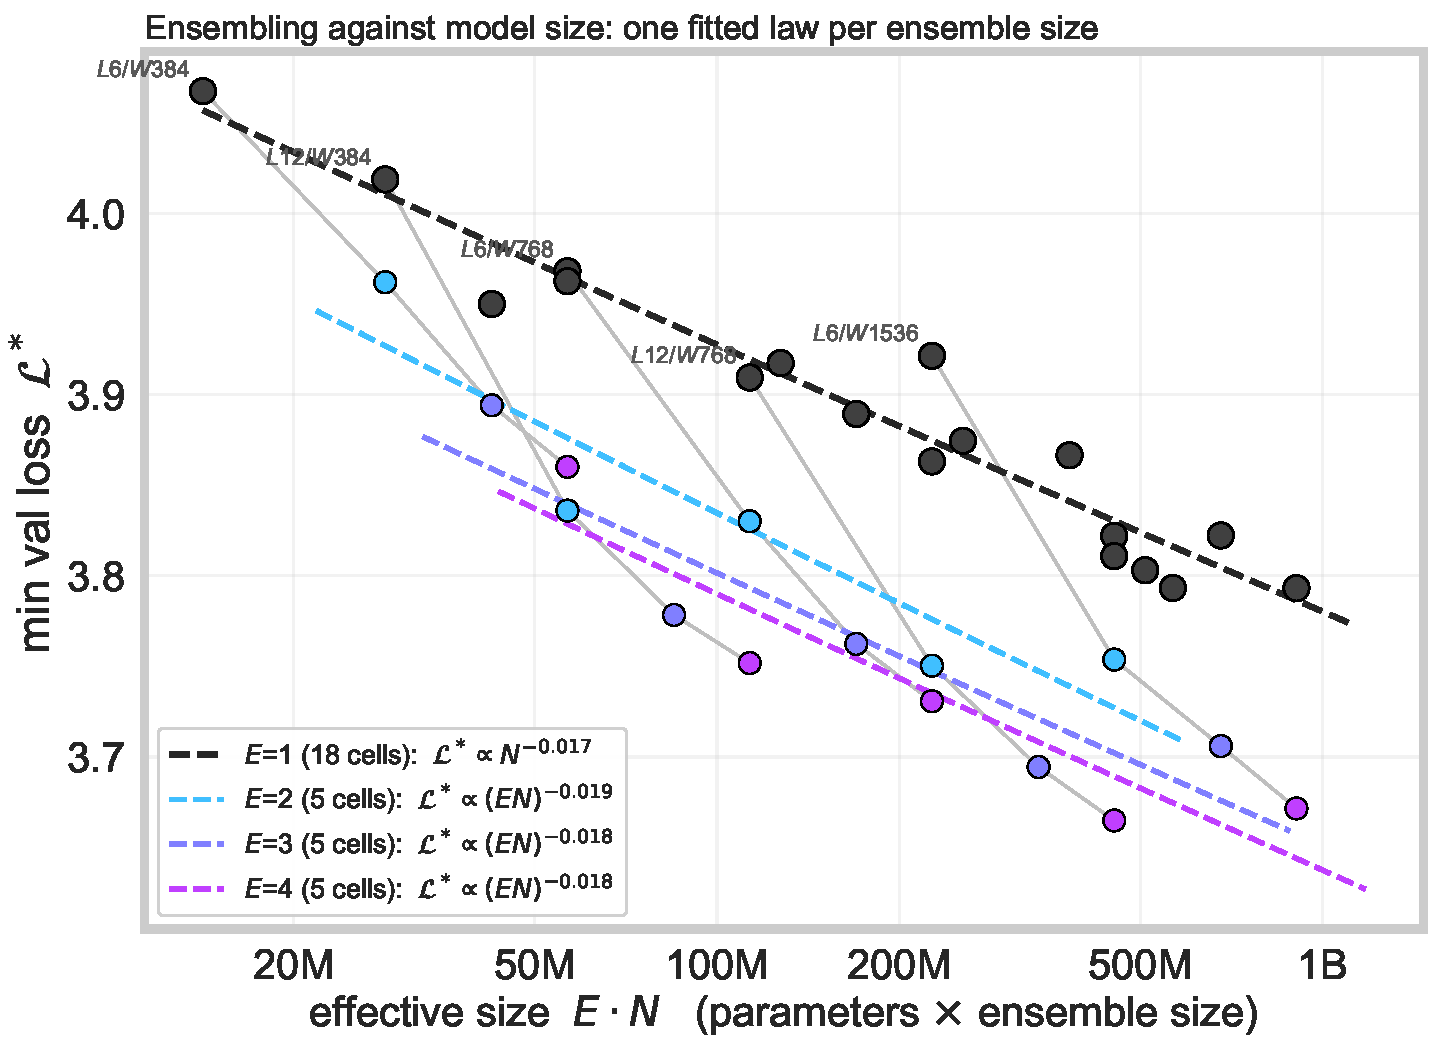
\includegraphics[width=\linewidth]{experiments/figures/11_ensemble_vs_size/expt_fig6_ensemble_vs_size.pdf}
  \caption{%
    Ensembling against model size at $P{=}100$M, $\lambda{=}0$. (A) Minimum
    validation loss against effective size $E\cdot N$; black circles and the
    dashed fit are the 12 single models, coloured markers are replayed ensembles
    of the four replicated cells (squares: $E{=}4$), arrows join each base model
    to its $4\times$ ensemble, and the solid line is the single-model law shifted
    down by the mean $E{=}4$ gap. (B) Gap below the single-model law for
    $E\in\{2,3,4,5\}$. (C) The same comparison against compute to the optimum.
  }
  \label{fig:ensemble_vs_size}
\end{figure}

% --- Notes ---
%
% Matched-size result (init_shuffle, min over the replayed curve):
%   L6/W384  x4 (57M)  3.8602  vs  L6/W768   3.9729   ensemble better by 0.113
%   L12/W384 x4 (113M) 3.7519  vs  L12/W768  3.9095                      0.158
%   L6/W768  x4 (226M) 3.7308  vs  L6/W1536  3.9323 / L24/W768 3.8728    0.20 / 0.14
%   L12/W768 x4 (453M) 3.6649  vs  L12/W1536 3.8221 / L48/W768 3.8257    0.16 / 0.16
%
% Shift vs new exponent: a uniform shift of 0.151 below the E=1 law has
% SSE 0.0020 over the four E=4 points; a shared-floor two-parameter fit gives
% alpha=0.42 (vs 0.19) with SSE 0.0008. Four points cannot separate these; the
% gap does grow slowly (0.117 -> 0.172 -> 0.146 -> 0.171), so "shifted down,
% widening slowly" is the defensible statement.
%
% Ensembles stop later: nadir epoch 30.9 vs 29.8, 26.9 vs 16.8, 17.9 vs 13.8,
% 13.9 vs 8.8 (E=4 vs its members).
%
% Floor vs data (expt_floor_vs_data.py), NOT in the manuscript because it is
% confounded: the only second corpus size with a model-size grid is the 20M
% 4x4 grid, which ran at lambda=0.1 with warmdown, against lambda=0 constant LR
% at 100M. What it does show: at 20M the minimum loss is FLAT in N (4.46-4.56
% over 14M-906M params; the saturating fit returns c<0), while at 100M the same
% span buys 0.30 nats. The additive prediction for the 20M floor,
% L_inf(100M)+[L*(20M)-L*(100M) at fixed model] = 3.54+0.83 = 4.37, sits below
% every 20M measurement (>= 4.46 at lambda=0.1; 4.74 at lambda=0 for the one
% cell we have), so the capacity term is not additive in P: it vanishes when
% the corpus is small relative to the model. A clean answer needs a lambda=0,
% constant-LR model-size ladder at a second P; at 20M that is ~1/4 the cost of
% the 100M cells.
